\subsection{Worker f�r Daten�bermittlung}\label{subsec:Worker}
Der vorliegende Abschnitt befasst sich mit dem Teil der Wissenserwerbskomponente, der als Bindeglied zwischen den Wissenserfassungsmethoden und der Wissensbasis auftritt und in Abbildung \ref{fig:wissenserwerbskomponente} als Schnittstelle f�r die Daten�bermittlung bezeichnet wird. Im Rahmen dieser Arbeit wird der Begriff \glqq{}\textit{Worker}\grqq{} verwendet, der f�r die Auspr�gung dieser Schnittstelle steht. Im Folgenden wird das Konzept hinter dem Worker abstrakt skizziert und im weiteren Verlauf mit der konkreten Implementierung verdeutlicht. Der Anwendungsbereich vom Worker l�sst sich in Abbildung \ref{fig:worker} wie folgt darstellen:
\begin{figure}[H] 
	\centering
	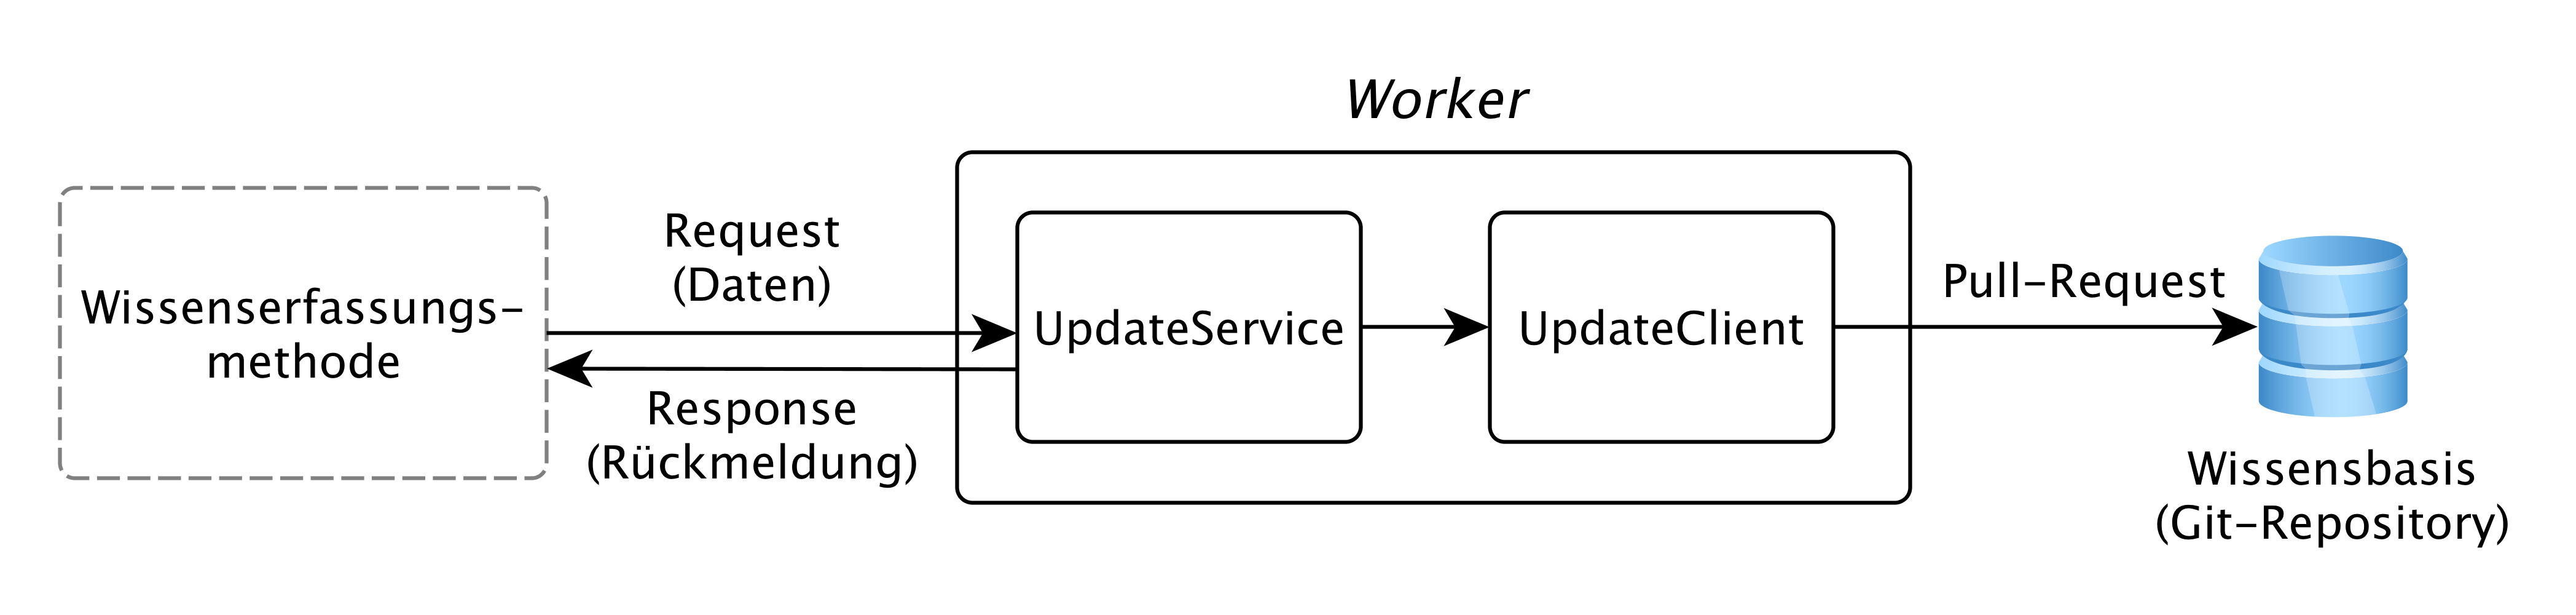
\includegraphics[width=1.0\textwidth]{images/anwendungsbereich_worker.png}
	\caption{Anwendungsbereich vom Worker}
	\label{fig:worker}
\end{figure}
Grunds�tzlich besteht der Worker aus zwei Komponenten, n�mlich \glqq{}\textit{UpdateService}\grqq{} und \glqq{}\textit{UpdateClient}\grqq{}. Die Aufgabe vom UpdateService besteht in der Bereitstellung einer Schnittstelle, die die Daten von au�en aufnimmt und die Daten�bermittlung an den UpdateClient delegiert. Auf der anderen Seite stellt der UpdateClient die Methoden zur Verf�gung, die f�r die Daten�bermittlung zust�ndig sind.\\
Generell l�sst sich der Ablauf gem�� der Abbildung \ref{fig:worker} folgenderma�en beschreiben. Als erstes werden die Daten von der Wissenserfassungsmethode an den UpdateService gesendet. Darauffolgend werden die Daten vom UpdateService verarbeitet und f�r den UpdateClient vorbereitet. Im n�chsten Schritt wird die Aufgabe der Daten�bermittlung an den UpdateClient delegiert. Der UpdateClient erstellt die Anfrage an die Wissensbasis und teilt die Antwort dem UpdateService mit. Anschlie�end verschickt der UpdateService die R�ckmeldung an die Wissenserfassungsmethode.\\ 
Technisch gesehen erfolgt der Nachrichtenaustausch zwischen Wissenserfassungsmethode, dem Worker und der Wissensbasis mithilfe von \ac{HTTP}\footnote{https://www.w3.org/Protocols}. F�r die weitere Betrachtung wird die Wissenstr�gerschnittstelle aus dem Abschnitt \ref{subsec:Wissenstr�gerschnittstelle} als Beispiel f�r die Wissenserfassungsmethode genommen. Die Wissensbasis stellt das Git-Repository von \textit{PaaSfinder} dar, das von einem Bot-Account auf Github \glqq{}geforkt\grqq{} wird\footnote{https://github.com/update-bot/paas-profiles}. In anderen Worten wird das urspr�ngliche Git-Repository von einem Account kopiert, der den schreibenden Zugriff auf die Wissensbasis hat.
%Als erstes werden die Daten als JSON an den UpdateService geschickt (Request). Im n�chsten Schritt wird das JSON vom UpdateService verarbeitet (\glqq{}geparsed\grqq{}{}) und die Pull-Request-Erstellung an den UpdateClient delegiert. An dieser Stelle wird davon ausgegangen, dass der Pull-Request erfolgreich erstellt wurde. Der genaue Ablauf der Pull-Request-Erstellung wird im sp�teren Verlauf detaillierter angesprochen. Nachdem der Pull-Request erstellt wurde, schickt der UpdateService eine R�ckmeldung (Response) an die Wissenserfassungsmethode.\\
%Technischbezogen erfolgt auf Basis von \ac{HTTP}\footnote{https://www.w3.org/Protocols} unter Verwendung von \ac{REST}-Architekturstil, der urspr�nglich aus der Dissertation von Fielding \cite{fielding2000} stammt. Das zentrale Konzept vom Rest besteht in Ressourcen, die im globalen Raum mithilfe von \ac{URI}\footnote{https://tools.ietf.org/html/rfc3986} eindeutig identifiziert werden \cite[S.11,35]{tilkov2015}. Ein wichtiges Merkmal von REST ist die lose Kopplung zwischen dem Client und dem Server, auch als statuslose Kommunikation bezeichnet \cite[S.18]{tilkov2015}. Der Server (Worker) interessiert sich f�r den Client (Wissenserfassungsmethode) nur f�r den Zeitpunkt der Request-Verarbeitung. Danach ist der Zustand des Clients f�r den Server nicht mehr relevant.\\
%Der UpdateService wird auf Basis Spark\footnote{http://sparkjava.com} umgesetzt. Spark stellt ein Micro-Framework dar, das eine kompakte, Java-basierte Implementierung von REST-API erm�glicht. Um die Daten von au�en empfangen zu k�nnen, stellt der UpdateService die \glqq{}/vendor\grqq{} Route zur Verf�gung, die vom Typ POST\footnote{https://tools.ietf.org/html/rfc7231\#section-4.3.3} ist und JSON als Medientyp erwartet.\\
%Die Erstellung eines Pull-Requests erfolgt mithilfe von Github REST-API\footnote{https://developer.github.com/v3}. Diese Aufgabe wird durch den UpdateClient durchgef�hrt und setzt sich aus folgenden Schritten zusammen:
%\begin{itemize}
%\item[1.] \acs{SHA}-Wert vom Master-Branch holen und einen neuen Branch erstellen
%\item[2.] \acs{SHA}-Wert der betroffenen JSON-Datei holen und die JSON-Datei innerhalb von Branch aktualisieren 
%\item[3.] einen Pull-Request erstellen
%\end{itemize}
%Diese Schritte werden der UpdateClient unter Verwendung von OkHttp\footnote{https://square.github.io/okhttp} implementiert und dem UpdateService als Methoden zur Verf�gung gestellt.\\
%Im folgenden Beispiel wird der Ablauf der Aktualisierung von dargestellt 
%\textit{Beispiel beschreiben}